\documentclass[11pt]{article}
\usepackage{parskip}
\usepackage[a4paper, total={7in, 10in}]{geometry}
\usepackage{amsmath,amsfonts,amsthm,bm}
\usepackage[english]{isodate}
\usepackage[final]{pdfpages}
\usepackage{graphicx} 
\usepackage{breakcites}
\usepackage{mathtools}
\usepackage{soul}
\usepackage{natbib}
\usepackage{authblk}
\usepackage[mathlines]{lineno}
\usepackage[labelfont=bf,skip=0.5cm,justification=justified,singlelinecheck=false]{caption}
\usepackage{outlines}
\bibliographystyle{agu}
%%%%%%%%%%%%%%%%%%%%%%%%%%%%%%%%%%%%%%%%%%%%%%%%%%%%%%%%%%%%%%%%%%%%%%%%%%%%%%%%%%%
%% Title %%%%%%%%%%%%%%%%%%%%%%%%%%%%%%%%%%%%%%%%%%%%%%%%%%%%%%%%%%%%%%%%%%%%%%%%%%
%%%%%%%%%%%%%%%%%%%%%%%%%%%%%%%%%%%%%%%%%%%%%%%%%%%%%%%%%%%%%%%%%%%%%%%%%%%%%%%%%%%
\title{Reliability of stock-recruitment function estimation in state space assessment models}
\author[1]{Gregory L. Britten}
\author[2]{Elizabeth Brooks}
\author[2]{Timothy Miller}
\affil[1]{Woods Hole Oceanographic Institution}
\affil[2]{Northeast Fisheries Science Center}
\date{\small{\printdayoff\today}}

\begin{document}
\maketitle 
\linenumbers
\section*{Abstract}
Stock-recruitment functions are important but difficult to estimate.

Many assessment models do not estimate stock-recruitment functions.

Maybe state space models help.

Here we ...

We find ...

This has implications for ...
%%%%%%%%%%%%%%%%%%%%%%%%%%%%%%%%%%%%%%%%%%%%%%%%%%%
%%%%%%%%%%%%%%%%%%%%%%%%%%%%%%%%%%%%%%%%%%%%%%%%%%%
\section*{Introduction}

%%%%%%%%%%%%%%%%%%%%%%%%%%%%%%%%%%%%%%%%%%%%%%%%%%%
%%%%%%%%%%%%%%%%%%%%%%%%%%%%%%%%%%%%%%%%%%%%%%%%%%%
\section*{Methods}
We used the WHAM package (ref, commit 77bbd94)

We performed a simulation study with 96 operating models that differed in the stock recruitment function used to simulate the population and a variety of additional variance parameter settings. 
Variance parameter settings were determined by a review of the range of estimates from recent applications of WHAM in management of stocks of haddock, butterfish, and American plaice in the NE US.

We simulated 100 data sets for each operating model. 

For each simulated data set we fit a set of 4 estimating models.

%%--OPERATING MODELS--%%
\subsubsection*{Operating Models}
The general operating model structure follows that of Project 0, reviewed briefly here. 
The population model tracks 10 age classes: ages 1 to 10+, assuming spawning occurs
1/4 of the way through the year. 
The maturity at age was a logistic curve with a50 = 2.89 and slope = 0.88, assumed known in all estimation models.

Weight at age was generated with a LVB growth function

$$ L_a = L_{\inf} \left( 1 - e^{-k(a-t_0}  \right)$$

with $t_0 = 0$, $L_{\inf}=85$, and $k=0.3$. The length-weight relationship is

$$W_a = \theta_1 L_a^{\theta_2}$$

with $\theta_1 = e^{-12.1}$ and $\theta_2 = 3.2$.

We assume a Beverton-Holt stock-recruitment of the form 

$$ N_{1,y} = \frac{\alpha\mathrm{SSB}_{y-1}}{1 + \beta \mathrm{SSB}_{y-1}} $$

where $\alpha$ is referred to as the density-independent recruitment and $\beta$ sets the strength of density-dependence. 
We specified unfished recruitment at $R_0 = e^{19}$ and $F_{MSY} = F_{\%40} = 0.348$ which corresponds to a steepness of 0.69, $\alpha=0.60$, and $\beta=2.4*10^{-5}$.

%%--ESTIMATING MODELS--%%
\subsubsection*{Estimating Models}


%%--ANALYSIS--%%
\subsubsection*{Analysis}

Metrics of interest: 
\begin{enumerate}
    \item Ability to correctly identify a stock recruitment relationship
    \item Ability correctly identify the functional form of the stock recruitment relationship
    \item Differences in estimation error (SSB, R) when SR relationships are correctly/incorrectly identified
\end{enumerate}

Generalized linear models

Generalized linear mixed models

Classification trees



%%%%%%%%%%%%%%%%%%%%%%%%%%%%%%%%%%%%%%%%%%%%%%%%%%%%%%%%%%%%%%%%%%%%%%%%%%%%%%%%%%%%%%%%%%%%%%%%%%%%%%%%%%%%%%%%
\section*{Results}

\begin{figure}[htb]
\begin{center}
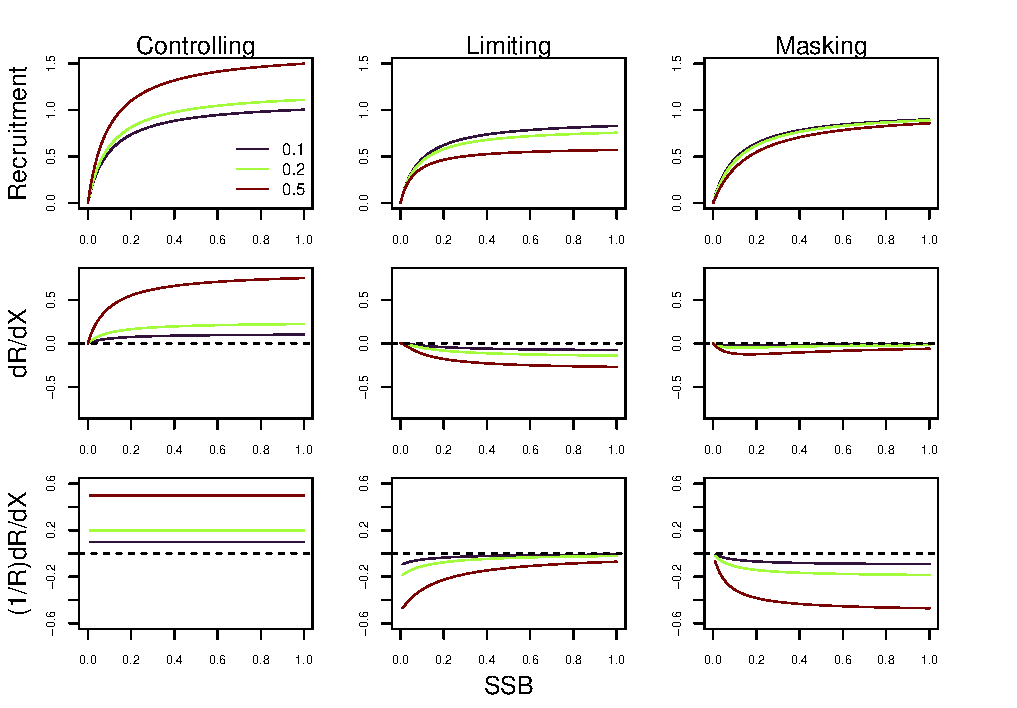
\includegraphics[width = 6in]{dRdX_1RdRdx.pdf}
\caption{Sensitivity of recruitment to environmental covariates for the three functional forms considered in this study.}
\end{center}
\end{figure}


\begin{figure}[htb]
\begin{center}
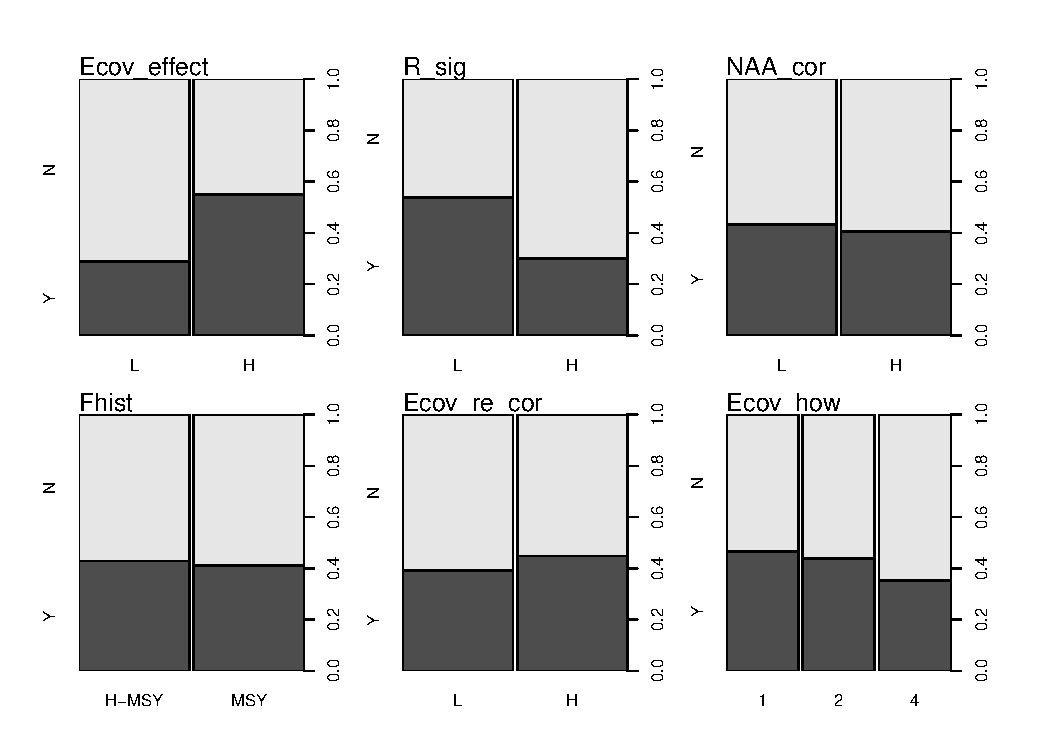
\includegraphics[width = 5in]{raw_boxplots_SR.pdf}
\caption{Model selection results for whether a stock recruitment relationship was correctly identified, expressed as marginal proportions against individual covariates.}
\end{center}
\end{figure}

\begin{figure}[htb]
\begin{center}
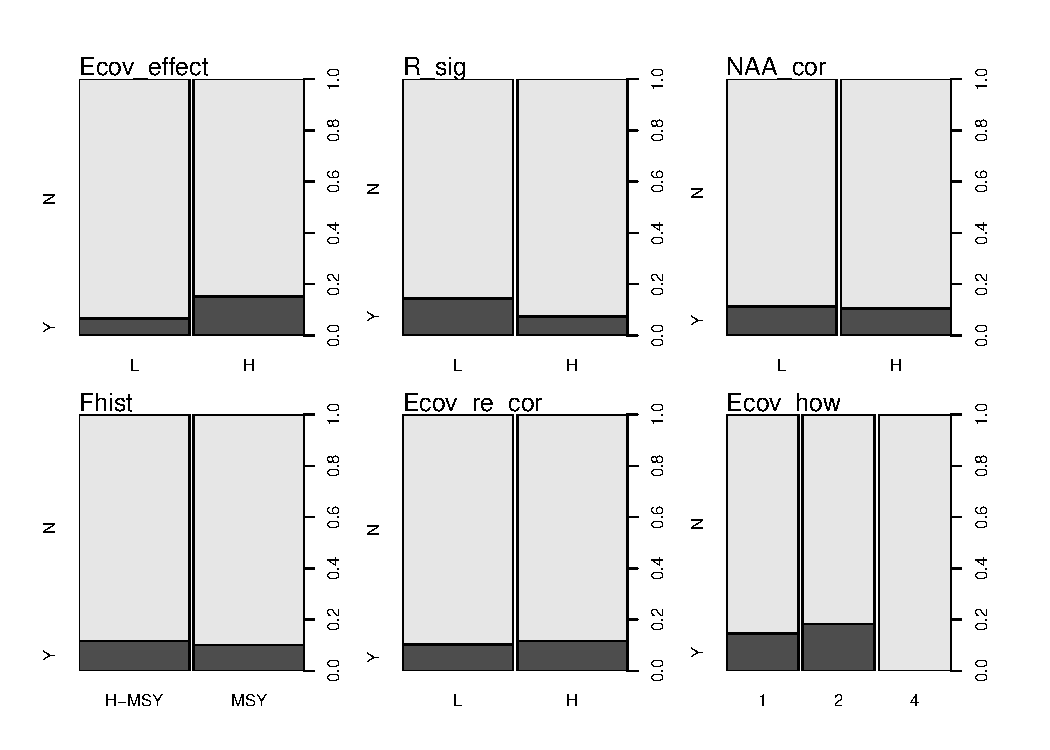
\includegraphics[width = 5in]{raw_boxplots_form.pdf}
\caption{Model selection results for whether the correct stock recruitment functional form was identified, expressed as marginal proportions against individual covariates.}
\end{center}
\end{figure}


\begin{figure}[htb]
\begin{center}
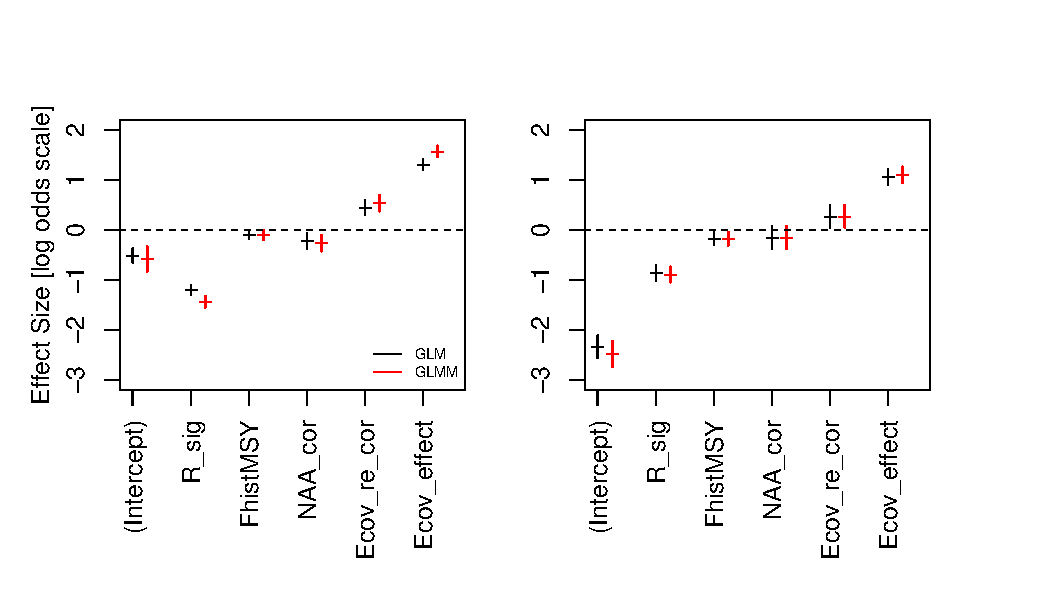
\includegraphics[width = 6in]{effect_size_glm_glmm.pdf}
\caption{Effect sizes for predicting estimated via a binomial generalized linear model and a binomial generalized linear mixed model with simulation random number seed as a random intercept.}
\end{center}
\end{figure}


\begin{figure}[htb]
\begin{center}
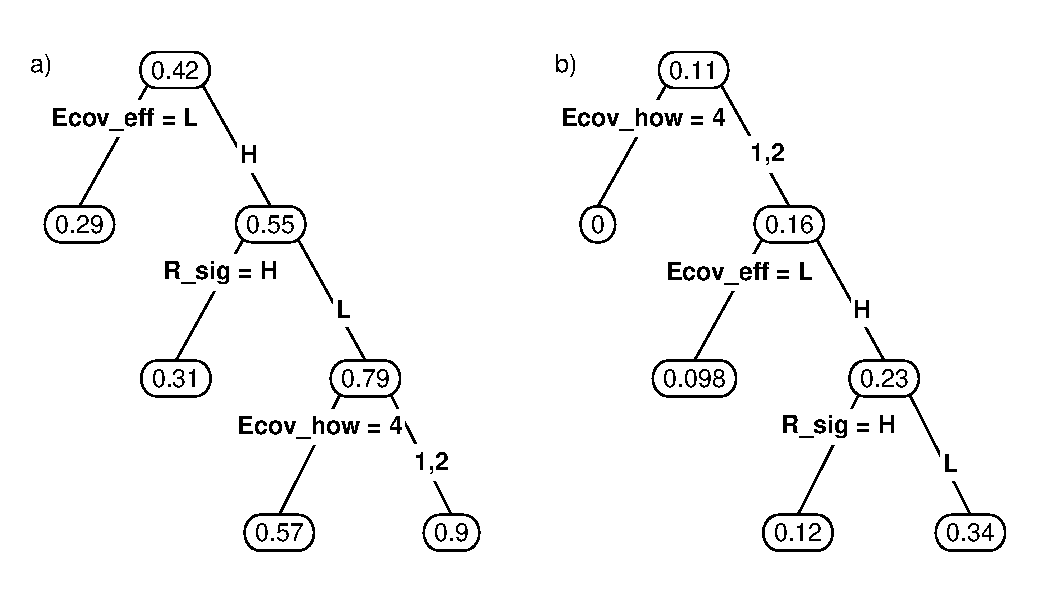
\includegraphics[width = 5in]{reg_tree.pdf}
\caption{Classification tree analysis of model selection results. R package `rpart' was used for the model fit and visualization. Following default settings in rpart, the complexity parameter is set at $c_p=0.01$ which represents the minimum classification improvement required for any split.}
\end{center}
\end{figure}



%%%%%%%%%%%%%%%%%%%%%%%%%%%%%%%%%%%%%%%%%%%%%%%%%%%%%%%%%%%%%%%%%%%%%%%%%%%%%%%%%%%%%%%%%%%%%%%%%%%%%%%%%%%%%%%%
\section*{Discussion}


%%%%%%%%%%%%%%%%%%%%%%%%%%%%%%%%%%%%%%%%%%%%%%%%%%%%%%%%%%%%%%%%%%%%%%%%%%%%%%%%%%%%%%%%%%%%%%%%%%%%%%%%%%%%%%%%
\section*{Appendix A}
% latex table generated in R 4.2.2 by xtable 1.8-4 package
% Wed Sep 13 13:05:00 2023
\begin{table}[ht]
\centering
\caption{Distinguishing characteristics of the operating models}
\resizebox{.65\textwidth}{!}{% <------ Don't forget this %
\begin{tabular}{rllrrlrlrrrr}
  \hline
 & Model & NAA\_re & Ecov\_obs\_sig & Ecov\_re\_sig & obs\_error & R\_sig & Fhist & NAA\_cor & Ecov\_re\_cor & Ecov\_effect & Ecov\_how \\ 
  \hline
1 & om\_1 & rec & 0.10 & 0.10 & L & 0.10 & H-MSY & 0.20 & 0.20 & 0.10 &   1 \\ 
  2 & om\_2 & rec & 0.10 & 0.10 & L & 1.00 & H-MSY & 0.20 & 0.20 & 0.10 &   1 \\ 
  3 & om\_3 & rec & 0.10 & 0.10 & L & 0.10 & MSY & 0.20 & 0.20 & 0.10 &   1 \\ 
  4 & om\_4 & rec & 0.10 & 0.10 & L & 1.00 & MSY & 0.20 & 0.20 & 0.10 &   1 \\ 
  5 & om\_5 & rec & 0.10 & 0.10 & L & 0.10 & H-MSY & 0.80 & 0.20 & 0.10 &   1 \\ 
  6 & om\_6 & rec & 0.10 & 0.10 & L & 1.00 & H-MSY & 0.80 & 0.20 & 0.10 &   1 \\ 
  7 & om\_7 & rec & 0.10 & 0.10 & L & 0.10 & MSY & 0.80 & 0.20 & 0.10 &   1 \\ 
  8 & om\_8 & rec & 0.10 & 0.10 & L & 1.00 & MSY & 0.80 & 0.20 & 0.10 &   1 \\ 
  9 & om\_9 & rec & 0.10 & 0.10 & L & 0.10 & H-MSY & 0.20 & 0.80 & 0.10 &   1 \\ 
  10 & om\_10 & rec & 0.10 & 0.10 & L & 1.00 & H-MSY & 0.20 & 0.80 & 0.10 &   1 \\ 
  11 & om\_11 & rec & 0.10 & 0.10 & L & 0.10 & MSY & 0.20 & 0.80 & 0.10 &   1 \\ 
  12 & om\_12 & rec & 0.10 & 0.10 & L & 1.00 & MSY & 0.20 & 0.80 & 0.10 &   1 \\ 
  13 & om\_13 & rec & 0.10 & 0.10 & L & 0.10 & H-MSY & 0.80 & 0.80 & 0.10 &   1 \\ 
  14 & om\_14 & rec & 0.10 & 0.10 & L & 1.00 & H-MSY & 0.80 & 0.80 & 0.10 &   1 \\ 
  15 & om\_15 & rec & 0.10 & 0.10 & L & 0.10 & MSY & 0.80 & 0.80 & 0.10 &   1 \\ 
  16 & om\_16 & rec & 0.10 & 0.10 & L & 1.00 & MSY & 0.80 & 0.80 & 0.10 &   1 \\ 
  17 & om\_17 & rec & 0.10 & 0.10 & L & 0.10 & H-MSY & 0.20 & 0.20 & 1.00 &   1 \\ 
  18 & om\_18 & rec & 0.10 & 0.10 & L & 1.00 & H-MSY & 0.20 & 0.20 & 1.00 &   1 \\ 
  19 & om\_19 & rec & 0.10 & 0.10 & L & 0.10 & MSY & 0.20 & 0.20 & 1.00 &   1 \\ 
  20 & om\_20 & rec & 0.10 & 0.10 & L & 1.00 & MSY & 0.20 & 0.20 & 1.00 &   1 \\ 
  21 & om\_21 & rec & 0.10 & 0.10 & L & 0.10 & H-MSY & 0.80 & 0.20 & 1.00 &   1 \\ 
  22 & om\_22 & rec & 0.10 & 0.10 & L & 1.00 & H-MSY & 0.80 & 0.20 & 1.00 &   1 \\ 
  23 & om\_23 & rec & 0.10 & 0.10 & L & 0.10 & MSY & 0.80 & 0.20 & 1.00 &   1 \\ 
  24 & om\_24 & rec & 0.10 & 0.10 & L & 1.00 & MSY & 0.80 & 0.20 & 1.00 &   1 \\ 
  25 & om\_25 & rec & 0.10 & 0.10 & L & 0.10 & H-MSY & 0.20 & 0.80 & 1.00 &   1 \\ 
  26 & om\_26 & rec & 0.10 & 0.10 & L & 1.00 & H-MSY & 0.20 & 0.80 & 1.00 &   1 \\ 
  27 & om\_27 & rec & 0.10 & 0.10 & L & 0.10 & MSY & 0.20 & 0.80 & 1.00 &   1 \\ 
  28 & om\_28 & rec & 0.10 & 0.10 & L & 1.00 & MSY & 0.20 & 0.80 & 1.00 &   1 \\ 
  29 & om\_29 & rec & 0.10 & 0.10 & L & 0.10 & H-MSY & 0.80 & 0.80 & 1.00 &   1 \\ 
  30 & om\_30 & rec & 0.10 & 0.10 & L & 1.00 & H-MSY & 0.80 & 0.80 & 1.00 &   1 \\ 
  31 & om\_31 & rec & 0.10 & 0.10 & L & 0.10 & MSY & 0.80 & 0.80 & 1.00 &   1 \\ 
  32 & om\_32 & rec & 0.10 & 0.10 & L & 1.00 & MSY & 0.80 & 0.80 & 1.00 &   1 \\ 
  33 & om\_33 & rec & 0.10 & 0.10 & L & 0.10 & H-MSY & 0.20 & 0.20 & 0.10 &   2 \\ 
  34 & om\_34 & rec & 0.10 & 0.10 & L & 1.00 & H-MSY & 0.20 & 0.20 & 0.10 &   2 \\ 
  35 & om\_35 & rec & 0.10 & 0.10 & L & 0.10 & MSY & 0.20 & 0.20 & 0.10 &   2 \\ 
  36 & om\_36 & rec & 0.10 & 0.10 & L & 1.00 & MSY & 0.20 & 0.20 & 0.10 &   2 \\ 
  37 & om\_37 & rec & 0.10 & 0.10 & L & 0.10 & H-MSY & 0.80 & 0.20 & 0.10 &   2 \\ 
  38 & om\_38 & rec & 0.10 & 0.10 & L & 1.00 & H-MSY & 0.80 & 0.20 & 0.10 &   2 \\ 
  39 & om\_39 & rec & 0.10 & 0.10 & L & 0.10 & MSY & 0.80 & 0.20 & 0.10 &   2 \\ 
  40 & om\_40 & rec & 0.10 & 0.10 & L & 1.00 & MSY & 0.80 & 0.20 & 0.10 &   2 \\ 
  41 & om\_41 & rec & 0.10 & 0.10 & L & 0.10 & H-MSY & 0.20 & 0.80 & 0.10 &   2 \\ 
  42 & om\_42 & rec & 0.10 & 0.10 & L & 1.00 & H-MSY & 0.20 & 0.80 & 0.10 &   2 \\ 
  43 & om\_43 & rec & 0.10 & 0.10 & L & 0.10 & MSY & 0.20 & 0.80 & 0.10 &   2 \\ 
  44 & om\_44 & rec & 0.10 & 0.10 & L & 1.00 & MSY & 0.20 & 0.80 & 0.10 &   2 \\ 
  45 & om\_45 & rec & 0.10 & 0.10 & L & 0.10 & H-MSY & 0.80 & 0.80 & 0.10 &   2 \\ 
  46 & om\_46 & rec & 0.10 & 0.10 & L & 1.00 & H-MSY & 0.80 & 0.80 & 0.10 &   2 \\ 
  47 & om\_47 & rec & 0.10 & 0.10 & L & 0.10 & MSY & 0.80 & 0.80 & 0.10 &   2 \\ 
  48 & om\_48 & rec & 0.10 & 0.10 & L & 1.00 & MSY & 0.80 & 0.80 & 0.10 &   2 \\ 
  49 & om\_49 & rec & 0.10 & 0.10 & L & 0.10 & H-MSY & 0.20 & 0.20 & 1.00 &   2 \\ 
  50 & om\_50 & rec & 0.10 & 0.10 & L & 1.00 & H-MSY & 0.20 & 0.20 & 1.00 &   2 \\ 
  51 & om\_51 & rec & 0.10 & 0.10 & L & 0.10 & MSY & 0.20 & 0.20 & 1.00 &   2 \\ 
  52 & om\_52 & rec & 0.10 & 0.10 & L & 1.00 & MSY & 0.20 & 0.20 & 1.00 &   2 \\ 
  53 & om\_53 & rec & 0.10 & 0.10 & L & 0.10 & H-MSY & 0.80 & 0.20 & 1.00 &   2 \\ 
  54 & om\_54 & rec & 0.10 & 0.10 & L & 1.00 & H-MSY & 0.80 & 0.20 & 1.00 &   2 \\ 
  55 & om\_55 & rec & 0.10 & 0.10 & L & 0.10 & MSY & 0.80 & 0.20 & 1.00 &   2 \\ 
  56 & om\_56 & rec & 0.10 & 0.10 & L & 1.00 & MSY & 0.80 & 0.20 & 1.00 &   2 \\ 
  57 & om\_57 & rec & 0.10 & 0.10 & L & 0.10 & H-MSY & 0.20 & 0.80 & 1.00 &   2 \\ 
  58 & om\_58 & rec & 0.10 & 0.10 & L & 1.00 & H-MSY & 0.20 & 0.80 & 1.00 &   2 \\ 
  59 & om\_59 & rec & 0.10 & 0.10 & L & 0.10 & MSY & 0.20 & 0.80 & 1.00 &   2 \\ 
  60 & om\_60 & rec & 0.10 & 0.10 & L & 1.00 & MSY & 0.20 & 0.80 & 1.00 &   2 \\ 
  61 & om\_61 & rec & 0.10 & 0.10 & L & 0.10 & H-MSY & 0.80 & 0.80 & 1.00 &   2 \\ 
  62 & om\_62 & rec & 0.10 & 0.10 & L & 1.00 & H-MSY & 0.80 & 0.80 & 1.00 &   2 \\ 
  63 & om\_63 & rec & 0.10 & 0.10 & L & 0.10 & MSY & 0.80 & 0.80 & 1.00 &   2 \\ 
  64 & om\_64 & rec & 0.10 & 0.10 & L & 1.00 & MSY & 0.80 & 0.80 & 1.00 &   2 \\ 
  65 & om\_65 & rec & 0.10 & 0.10 & L & 0.10 & H-MSY & 0.20 & 0.20 & 0.10 &   4 \\ 
  66 & om\_66 & rec & 0.10 & 0.10 & L & 1.00 & H-MSY & 0.20 & 0.20 & 0.10 &   4 \\ 
  67 & om\_67 & rec & 0.10 & 0.10 & L & 0.10 & MSY & 0.20 & 0.20 & 0.10 &   4 \\ 
  68 & om\_68 & rec & 0.10 & 0.10 & L & 1.00 & MSY & 0.20 & 0.20 & 0.10 &   4 \\ 
  69 & om\_69 & rec & 0.10 & 0.10 & L & 0.10 & H-MSY & 0.80 & 0.20 & 0.10 &   4 \\ 
  70 & om\_70 & rec & 0.10 & 0.10 & L & 1.00 & H-MSY & 0.80 & 0.20 & 0.10 &   4 \\ 
  71 & om\_71 & rec & 0.10 & 0.10 & L & 0.10 & MSY & 0.80 & 0.20 & 0.10 &   4 \\ 
  72 & om\_72 & rec & 0.10 & 0.10 & L & 1.00 & MSY & 0.80 & 0.20 & 0.10 &   4 \\ 
  73 & om\_73 & rec & 0.10 & 0.10 & L & 0.10 & H-MSY & 0.20 & 0.80 & 0.10 &   4 \\ 
  74 & om\_74 & rec & 0.10 & 0.10 & L & 1.00 & H-MSY & 0.20 & 0.80 & 0.10 &   4 \\ 
  75 & om\_75 & rec & 0.10 & 0.10 & L & 0.10 & MSY & 0.20 & 0.80 & 0.10 &   4 \\ 
  76 & om\_76 & rec & 0.10 & 0.10 & L & 1.00 & MSY & 0.20 & 0.80 & 0.10 &   4 \\ 
  77 & om\_77 & rec & 0.10 & 0.10 & L & 0.10 & H-MSY & 0.80 & 0.80 & 0.10 &   4 \\ 
  78 & om\_78 & rec & 0.10 & 0.10 & L & 1.00 & H-MSY & 0.80 & 0.80 & 0.10 &   4 \\ 
  79 & om\_79 & rec & 0.10 & 0.10 & L & 0.10 & MSY & 0.80 & 0.80 & 0.10 &   4 \\ 
  80 & om\_80 & rec & 0.10 & 0.10 & L & 1.00 & MSY & 0.80 & 0.80 & 0.10 &   4 \\ 
  81 & om\_81 & rec & 0.10 & 0.10 & L & 0.10 & H-MSY & 0.20 & 0.20 & 1.00 &   4 \\ 
  82 & om\_82 & rec & 0.10 & 0.10 & L & 1.00 & H-MSY & 0.20 & 0.20 & 1.00 &   4 \\ 
  83 & om\_83 & rec & 0.10 & 0.10 & L & 0.10 & MSY & 0.20 & 0.20 & 1.00 &   4 \\ 
  84 & om\_84 & rec & 0.10 & 0.10 & L & 1.00 & MSY & 0.20 & 0.20 & 1.00 &   4 \\ 
  85 & om\_85 & rec & 0.10 & 0.10 & L & 0.10 & H-MSY & 0.80 & 0.20 & 1.00 &   4 \\ 
  86 & om\_86 & rec & 0.10 & 0.10 & L & 1.00 & H-MSY & 0.80 & 0.20 & 1.00 &   4 \\ 
  87 & om\_87 & rec & 0.10 & 0.10 & L & 0.10 & MSY & 0.80 & 0.20 & 1.00 &   4 \\ 
  88 & om\_88 & rec & 0.10 & 0.10 & L & 1.00 & MSY & 0.80 & 0.20 & 1.00 &   4 \\ 
  89 & om\_89 & rec & 0.10 & 0.10 & L & 0.10 & H-MSY & 0.20 & 0.80 & 1.00 &   4 \\ 
  90 & om\_90 & rec & 0.10 & 0.10 & L & 1.00 & H-MSY & 0.20 & 0.80 & 1.00 &   4 \\ 
  91 & om\_91 & rec & 0.10 & 0.10 & L & 0.10 & MSY & 0.20 & 0.80 & 1.00 &   4 \\ 
  92 & om\_92 & rec & 0.10 & 0.10 & L & 1.00 & MSY & 0.20 & 0.80 & 1.00 &   4 \\ 
  93 & om\_93 & rec & 0.10 & 0.10 & L & 0.10 & H-MSY & 0.80 & 0.80 & 1.00 &   4 \\ 
  94 & om\_94 & rec & 0.10 & 0.10 & L & 1.00 & H-MSY & 0.80 & 0.80 & 1.00 &   4 \\ 
  95 & om\_95 & rec & 0.10 & 0.10 & L & 0.10 & MSY & 0.80 & 0.80 & 1.00 &   4 \\ 
  96 & om\_96 & rec & 0.10 & 0.10 & L & 1.00 & MSY & 0.80 & 0.80 & 1.00 &   4 \\ 
   \hline
\end{tabular}
}
\end{table}

% latex table generated in R 4.2.2 by xtable 1.8-4 package
% Wed Sep 13 13:08:37 2023
\begin{table}[ht]
\centering
\begin{tabular}{rrl}
  \hline
 & ecov\_how & r\_mod \\ 
  \hline
1 &   0 & BH \\ 
  2 &   1 & BH \\ 
  3 &   2 & BH \\ 
  4 &   4 & BH \\ 
   \hline
\end{tabular}
\end{table}




\bibliography{refs.bib}
 
\end{document}